\documentclass[a4paper]{article}

\usepackage{tikz}
\usetikzlibrary{shapes.geometric, arrows, calc, positioning}
\tikzstyle{process} = [rectangle, minimum width=4cm, minimum height=1cm, text centered, draw=black, fill=orange!30]
\tikzstyle{decision} = [rectangle, minimum width=3cm, minimum height=1cm, text centered, draw=black, fill=green!30]
\tikzstyle{stop} = [rectangle, minimum width=1.5cm, minimum height=1cm, text centered, draw=black, fill=red!30]
\tikzstyle{arrow} = [thick,->,>=stealth]
\tikzstyle{line} = [draw,thick,->,-latex',>=stealth]

\title{remotePLC v1.0\\User's and Programmer's Guide}
\author{Christian A. Schmitz - christian.schmitz@telenet.be}

\begin{document}
\maketitle
\newpage
\tableofcontents
\newpage
\part{User's Guide}
\section{Synopsis}
\textit{remotePLC} is a ``soft'' PLC (Programmable Logic Controller). This means that it runs on a computer and connects to sensors and actuators via ethernet or other IOs. \textit{remotePLC} is designed as a utility to interface with the \textit{Internet-of-Things} (hence ``\textit{remote}''), although it can also interface with conventional PLC devices depending on the available IOs.\\\\
The user specifies input blocks, logic blocks, and output blocks via command-line or a configuration file. These blocks process data in the form of arrays of double precision numbers. This data is moved between the blocks via lines, which also need to be specified by the user.\\\\
Finally the user specifies the criteria that end the program (e.g. stop the program after 10min, or stop when certain stability conditions are reached).\\\\
\textit{remotePLC} then reads the provided statements and constructs a graph. After connectivity checks the input blocks are launched in an infinite update loop (running in the background), and the main PLC loop is started. Figure \ref{fig:basic_flowchart} shows a flowchart of the \textit{remotePLC} processes.
\begin{figure}
  \center
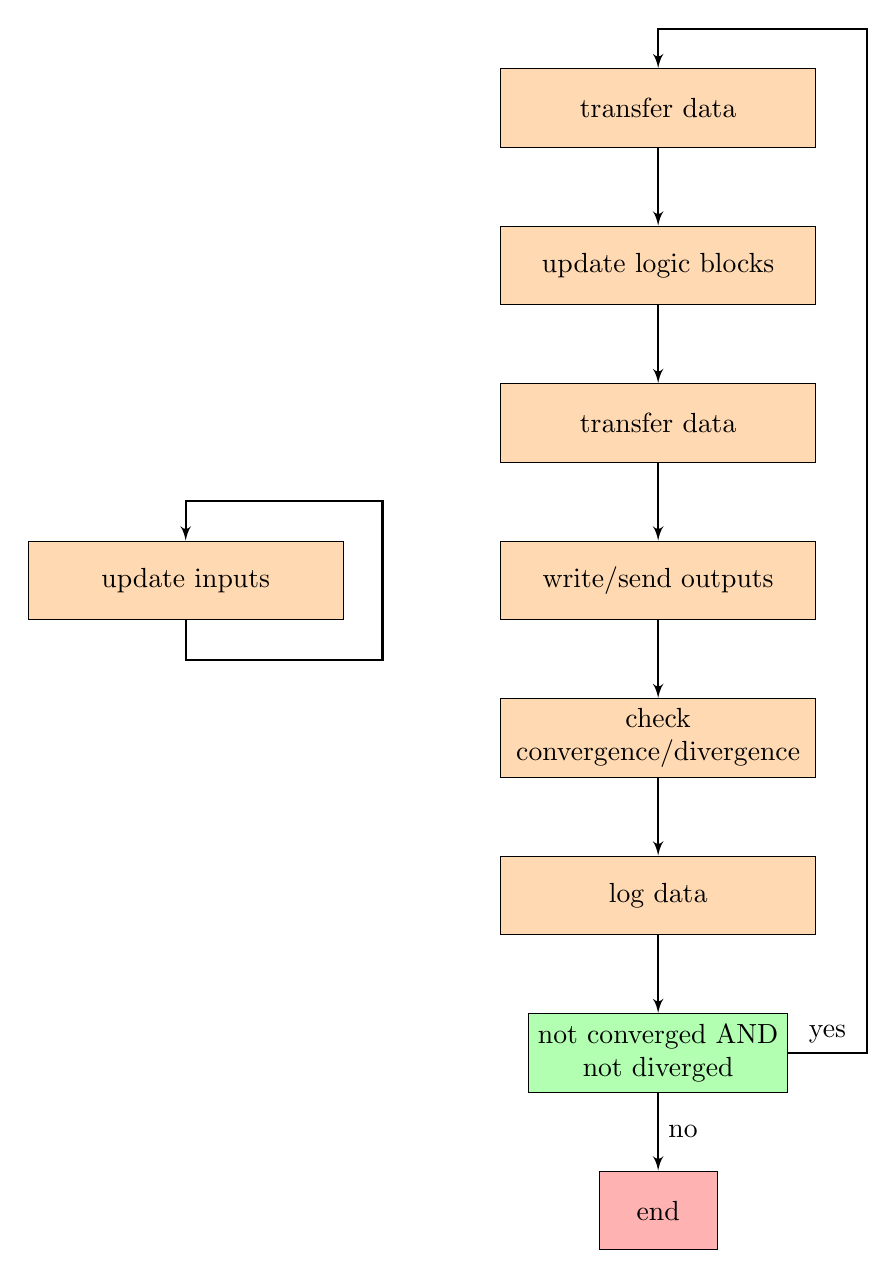
\begin{tikzpicture}[node distance=2cm]
  \node (inputs) [process, xshift=-3cm, yshift=-6cm] {update inputs};
  \path [line] (inputs.south) |- ($(inputs.south) + (2.5,-0.5)$) |- ($(inputs.north) + (2.5,0.5)$) -- ($(inputs.north) + (0.0,0.5)$) -- (inputs.north);

  \node (move1) [process, xshift=3cm, yshift=0cm] {transfer data};

  \node (logic) [process, xshift=3cm, yshift=-2cm] {update logic blocks};
  \path [line] (move1) -- (logic);

  \node (move2) [process, xshift=3cm, yshift=-4cm] {transfer data};
  \path [line] (logic) -- (move2);

  \node (outputs) [process, xshift=3cm, yshift=-6cm] {write/send outputs};
  \path [line] (move2) -- (outputs);

  \node (convergence) [process, align=center, xshift=3cm, yshift=-8cm] {check\\convergence/divergence};
  \path [line] (outputs) -- (convergence);

  \node (log) [process, xshift=3cm, yshift=-10cm] {log data};
  \path [line] (convergence) -- (log);

  \node (while) [decision, xshift=3cm, yshift=-12cm, align=center] {not converged AND \\not diverged};
  \path [line] (log) -- (while);

  \node (end) [stop, xshift=3cm, yshift=-14cm] {end};
  \path [line] (while.east) -- node[anchor=south] {yes} ($(while.east) + (1.0,0.0)$) |- ($(move1.north) + (0.0, 0.5)$) -- (move1);
  \path [line] (while) -- node[anchor=west] {no} (end);
\end{tikzpicture}
\caption{flowchart of the \textit{remotePLC} processes}
\label{fig:basic_flowchart}
\end{figure}
\section{Block types}
\subsection{Input types}
\subsubsection{ConstantInput}
Declared as: name ConstantInput 1.0\\\\
Arrays are possible by specifying additional numbers.
\subsubsection{FileInput}
Declared as: name FileInput fname\\\\
The file is reread every time step. So it can be used as a runtime modifiable input.
Rows and columns don't matter, all individual numbers are read into an array. (by row first, then next row etc.)
\subsubsection{ScaleInput}
Declared as: name ScaleInput scale offset OtherInputType $\ldots$\\\\
Immediately applies a scale-factor and an offset to all the doubles gotten from the OtherInputType.
\subsubsection{TimeFileInput}
Declared as: name TimeFileInput fname\\\\
Reread when changed. First column is the time in seconds. Between two rows the result is gotten via linear interpolation. If one row contains more numbers than the other, then the other is copied locally, and completed with zeros, before interpolation.
\subsubsection{ZeroInput}
Declared as: name ZeroInput\\\\
Identical to: name ConstantInput 0.0
\subsubsection{ExampleUDPInput}
Not functional code, just provided as a template for implementing the sensor side of your own UDP protocol.
\subsection{Output types}
\subsubsection{FileOutput}
Declared as: name FileOutput fname\\\\
Writes the numbers as a column to fname. Can also be stdout or stderr.
File seeks to 0th position every time step though, so this can't be used for logging.
\subsubsection{PhilipsHueBridgeOutput}
Declared as: name PhilipsHueBridgeOutput ipaddr userkey lightNo\\\\
See tutorial/philipsHue on how to determine the ipaddr and userkey for your philips hue bridge.
This output sets the brightness of the light if only one number is given, the brightness and hue if two numbers are specified, the brightness hue and saturation if 3 numbers are specified. All 3 are numbers between 0 and 1. Negative brightness turns off the light, above 1.0 is clipped. Hue values above 1.0 are wrapped around to 0.0 (and negative is wrapped to 1.0). Saturation values are clipped to lie between 0.0 and 1.0 inclusive. The clipping/wrapping behaviour is done internally and not visible to the user.
\subsubsection{ExampleUDPOutput}
Not functional code, just provided as a template for implementing the actuator side of your own UDP protocol.
\subsection{Lines}
\subsubsection{Line}
Declared as: name Line in1 out1 in2 out2\\\\
Simply move data from in to out. Any number of pairs is possible. Unpaired lines throw an error.
\subsubsection{DiffLine}
Declared as: name DiffLine in1 in2 out\\\\
$out = in2 - in1$. If the input arrays have a different length then the longest is clipped to the shortest length.
\subsubsection{ForkLine}
Declared as: name ForkLine in out1 out2 out3 out4 \ldots\\\\
Copy $in$ to all the specified outputs. Any number of outputs is possible.
\subsubsection{JoinLine}
Declared as: name JoinLine out in1 in2 in3 in4 \ldots\\\\
Concatenate all the arrays from all the inputs and send to $out$. Any number of inputs is possible.
\subsubsection{RegexpForkLine}
Create a ForkLine where the output list is created by matching a regexp on the names of other blocks.
\subsubsection{RegexpJoinLine}
Create a JoinLine where the input list is created by matching a regexp on the names of other blocks.
\subsubsection{RegexpLine}
Create a Line by matching regexp on all the blocks in order to determine the pairs. Unpaired in or outputs are ignored.
\subsubsection{SplitLine}
Declared as: name SplitLine 1 in out1 out2 out3 \_ out5\\\\
Split the input array in <size>-parts and send each section to a corresponding output. The underscore means that that section is ignored.
\subsection{Logic}
TODO: Selfoptimizing PID blocks.
\subsubsection{DelayLogic}
Declared as: name DelayLogic\\\\
Incoming data is simply moved to the outgoing side.
\subsubsection{PIDLogic}
Declared as: name PIDLogic KP KI KD\\\\
Keeps track of the previous time step error and error integral. Input to this is the error! and not the setpoint value. You will need to do a diffline before this block. TODO: when the program stops the state is lost, it would probably be best to store this state in a file, so that the program can resume smoothly. This means that the simple kill signals needs to be caught and give the program time to complete the saving of the state.\\
\subsection{Nodes}
These blocks copy their input directly to their outputs. There is no update step. This useful when you want to propagate the most recent value downstream.
\subsubsection{LimitNode}
Declared as: name LimitNode 0.0 1.0\\\\
Clips all elements of the input array so they lie between these two numbers.
\subsubsection{Node}
Declared as: name Node\\\\
Copy upstream values immediately downstream.
\subsubsection{ScaleNode}
Like ScaleInput: name ScaleNode scale offset\\\\
\subsubsection{BitifyNode}
Convert each input into a 0 or 1 and then multiply by corresponding power of 2. Output is a single number representing the uint resulting value.
\subsection{Stop}
A number <= -1 means that the stop block is converged. A number between -1 and <= 1 means that the stop block is neither converged or diverged. A number above 1 means that the block is diverging. The program stop if all blocks are converged, or if one block is diverging. If there are no stop blocks defined then the program exits immediately.
\subsubsection{TimeOutStop}
Declared as: name TimeOutStop duration\\\\
duration is a string that is parsed. (see go/pkg/time documentation). So this means that the program is ``diverging'' after <duration>.
\subsubsection{TimeStop}
Declared as: name TimeStop duration\\\\
Program is ``converging'' after <duration>.
\section{TODO}
Still a primitive program. Send recommendations to christian.schmitz@telenet.be
Does anything like this exist? (in that case: sorry for duplicating any one elses efforts)
\begin{itemize}
  \item anonymous blocks (autogeneration of name for use in internal map date structures)
  \item piping notation for sequential blocks, so the the lines don't always need to be specified manually
  \item multiline statements in blocks.cfg
  \item semicolon parsing in blocks.cfg
\end{itemize}
\section{License}
MIT, see LICENSE.txt included in source code package.
\part{Programmer's Guide}
\section{Background: motivation}
I couldn't find a PLC with the following specs, and thus wrote \textit{remotePLC}:
\begin{itemize}
  \item FOSS
  \item text or command-line based
  \item no recompilation in case of a new graph
\end{itemize}
Each of these points is very important to me. (I leave it up to you to guess which PLC-like software does NOT have these properties and frustrated me up to the point to start writing \textit{remotePLC} in my free time).
\subsection{FOSS}
License fees are a pain, no matter how small. You just want to depend as little as possible on any purchase approval procedures at your company. The bureaucracy could slow you down immensely. I estimate that my (free) time spent writing the first functional version of \textit{remotePLC} is probably less than the time I would've wasted on the bureaucracy for a commercial alternative (not to mention the amount of frustration saved).
\subsection{Text or command-line based}
This has two advantages: automation and ssh. I can call \textit{remotePLC} from a higher level script and run the whole thing remotely on very simple computers. My original goal was actually to use \textit{Dakota} to do Designs of Experiments and run advanced optimization algorithms on a remote industrial pc.\\\\
I guess this could be possible with commercial alternatives, but I imagine the interfacing overhead being somewhat more complex.
\subsection{No recompilation}
The remote industrial computers I want to run \textit{remotePLC} on might not have compilers installed. And at some point in the future I will hopefully even forget how to compile \textit{remotePLC}. So I want to avoid recompilation by providing enough flexibility through a configuration file.\\\\
But at the same time I want to avoid that the configuration file itself becomes a meta-program, and thus non-trivial to use. This requires the right balance between the functionality of the program and the configuration file.
\section{General structure}
Arrays of double precision numbers are passed between the blocks via the ``lines''.
Time loop:
\begin{itemize}
  \item inputs are cycled in the background (default 250ms, 10ms desyncing between each input). So the input cycle is NOT in sync with the rest of the program.
  \item lines are updated (serially)
  \item logic is updated (serially) 
  \item lines are updated again (serially) , so that outputs are sure to get the needed values 
  \item outputs are cycled (in parallel, forked and joined)
  \item the stop criteria are cycled (serially)
  \item data is logged
\end{itemize}
This is not a high performance plc program, and I'm not sure how it will behave in case of very short time loops. 1ms should be doable though, although most IO probably has higher latency.
\subsection{Modules and Files}
In more or less chronological call order:
\begin{itemize}
  \item main::remotePLC.go: parse args, read blocks, construct blocks, start controlLoop, COMMENT\_CHAR, EXTRA\_NEWLINE\_CHAR
  \item main::controlLoop.go: order lines, check connectivity, get inputs once, start cycling inputs in background, start main time loop, log data once before exiting
  \item main::controlLoop.go.mainTimeLoop: cycle lines, cycle logic, cycle lines, cycle outputs, cycle stoppers, logdata
  \item blocks::blocks.go: Blocks map, constructor map, input/basic/output structs/interfaces, get blocks, add and get constructors, construct block, LogData(), BlockModeType=REGULAR,CONNECTIVITY,STRICT, HIDDEN\_SUFFIX\_CHAR
  \item blocks::*: dynamically constructed blocks with Get(), Put(), and Update() functions
  \item logger::eventLogger.go: EventModeType=QUIET,WARNING,FATAL, WriteEvents(), WriteError()
  \item logger::dataLogger.go: headerPrefix, fnameFormat/regexp, maxFileSize, maxTotalSize, WriteData()
\end{itemize}
\end{document}


